\documentclass[
	% -- opções da classe memoir --
	12pt,				% tamanho da fonte
	openany,			% capítulos começam em pág ímpar (insere página vazia caso preciso)
  oneside,      % para impressão em página única. Oposto ao twoside (Nunca habilitar os dois!)
	%twoside,			% para impressão em recto e verso. Oposto a oneside (Nunca habilitar os dois!)
	a4paper,			% tamanho do papel. 
	% -- opções da classe abntex2 --
	%chapter=TITLE,		% títulos de capítulos convertidos em letras maiúsculas
	%section=TITLE,		% títulos de seções convertidos em letras maiúsculas
	%subsection=TITLE,	% títulos de subseções convertidos em letras maiúsculas
	%subsubsection=TITLE,% títulos de subsubseções convertidos em letras maiúsculas
	% -- opções do pacote babel --
	english,			% idioma adicional para hifenização
	french,				% idioma adicional para hifenização
	spanish,			% idioma adicional para hifenização
	brazil				% o último idioma é o principal do documento
	]{abntex2}

% ---
% Pacotes básicos 
% ---
\usepackage{lmodern}			  % Usa a fonte Latin Modern			
\usepackage[T1]{fontenc}		% Selecao de codigos de fonte.
\usepackage[utf8]{inputenc} % Codificacao do documento (conversão automática dos acentos)
\usepackage{lastpage}			  % Usado pela Ficha catalográfica
\usepackage{indentfirst}    % Indenta o primeiro parágrafo de cada seção.
\usepackage{color}				  % Controle das cores
\usepackage{graphicx}			  % Inclusão de gráficos
\usepackage{subfig}         % Sub-figuras
\usepackage{microtype}      % para melhorias de justificação
\usepackage{textcomp}       % Adiciona símbolo de trademark e outros ao T1
\usepackage{array}          % Usado nas tabelas com \newline
\usepackage{multirow}       % Define tabelas multirow
\usepackage[outputdir=Gen]{minted}
\usepackage{listings}       % Program listings
\usepackage{lscape}         % 90-degree rotated images and tables
\usepackage{longtable}      % multiple pages tables
\usepackage{booktabs}       % http://ctan.org/pkg/booktabs
		
% ---
% Pacotes adicionais, usados apenas no âmbito do Modelo Canônico do abnteX2
% ---
\usepackage{lipsum}				% para geração de dummy text
% ---

% ---
% Pacotes de citações
% ---
\usepackage[brazilian,hyperpageref]{backref}	 % Paginas com as citações na bibl
\usepackage[alf]{abntex2cite}	% Citações padrão ABNT

% Copiado das configurações do LyX

%%%%%%%%%%%%%%%%%%%%%%%%%%%%%% LyX specific LaTeX commands.
%% Because html converters don't know tabularnewline
\providecommand{\tabularnewline}{\\}

%%%%%%%%%%%%%%%%%%%%%%%%%%%%%% User specified LaTeX commands.

% --- 
% CONFIGURAÇÕES DE PACOTES
% --- 

% ---
% Configurações do pacote backref
% Usado sem a opção hyperpageref de backref
\renewcommand{\backrefpagesname}{Citado na(s) página(s):~}
% Texto padrão antes do número das páginas
\renewcommand{\backref}{}
% Define os textos da citação
\renewcommand*{\backrefalt}[4]{
	\ifcase #1 %
		Nenhuma citação no texto.%
	\or
		Citado na página #2.%
	\else
		Citado #1 vezes nas páginas #2.%
	\fi}%
% ---

% Adiciona fake itemize for tabitem
\newcommand{\tabitem}{~~\llap{\textbullet}~~}

% ---
% nomes
\newcommand{\nomeDoBanco}{Banco Bolinha SA}
\newcommand{\nomeCompletoPositivo}{Positivo Tecnologia SA}
\newcommand{\nomePositivo}{Positivo Tecnologia}
\newcommand{\nomePositivoAr}{Positivo BGH}
% ---


% ---
% Informações de dados para CAPA e FOLHA DE ROSTO
% ---
\titulo{Análise \nomeCompletoPositivo}

\autor{André Ferreira Bem Silva \\ Augusto Gonçalves \\ Fernando D'Império \\ Kleber Daniel \\ Marcos Vinício Siqueira \\ William Dantas }

\local{São Paulo, SP}
\data{18/08/2018}
\instituicao{%
  Fundação Getúlio Vargas -- FGV
  \par
  MBA Executivo em Economia e Gestão: Business Analytics e Big Data T3
  \par
  Disciplina de Controladoria Gerencial
}
\tipotrabalho{Resenha}
% O preambulo deve conter o tipo do trabalho, o objetivo, 
% o nome da instituição e a área de concentração 
\preambulo{Este trabalho trata-se de uma análise do banco de investimentos \nomeDoBanco. }
% ---


% ---
% Configurações de aparência do PDF final

% alterando o aspecto da cor azul
\definecolor{blue}{RGB}{41,5,195}

% informações do PDF
\makeatletter
\hypersetup{
     	%pagebackref=true,
		pdftitle={\@title}, 
		pdfauthor={\@author},
    	pdfsubject={\imprimirpreambulo},
	    pdfcreator={LaTeX with abnTeX2},
		pdfkeywords={abnt}{latex}{abntex}{abntex2}{trabalho acadêmico}, 
		colorlinks=true,       		% false: boxed links; true: colored links
    	linkcolor=blue,          	% color of internal links
    	citecolor=blue,        		% color of links to bibliography
    	filecolor=magenta,      		% color of file links
		urlcolor=blue,
		bookmarksdepth=4
}
\makeatother
% --- 

% --- 
% Espaçamentos entre linhas e parágrafos 
% --- 

% O tamanho do parágrafo é dado por:
\setlength{\parindent}{1.3cm}

% Controle do espaçamento entre um parágrafo e outro:
\setlength{\parskip}{0.2cm}  % tente também \onelineskip

% ---
% compila o indice
% ---
\makeindex
% ---

% ----
% Início do documento
% ----
\begin{document}

% Seleciona o idioma do documento (conforme pacotes do babel)
%\selectlanguage{english}
\selectlanguage{brazil}

% Retira espaço extra obsoleto entre as frases.
\frenchspacing 

% ----------------------------------------------------------
% ELEMENTOS PRÉ-TEXTUAIS
% ----------------------------------------------------------
% \pretextual

% ---
% Capa
% ---
\imprimircapa
% ---

% ---
% Folha de rosto
% (o * indica que haverá a ficha bibliográfica)
% ---
\imprimirfolhaderosto
% ---

% ---

% ---

% ---

% ---
% inserir lista de ilustrações
% ---
\pdfbookmark[0]{\listfigurename}{lof}
\listoffigures*
\cleardoublepage
% ---

% ---
% inserir lista de tabelas
% ---
\pdfbookmark[0]{\listtablename}{lot}
\listoftables*
\cleardoublepage
% ---

% ---
% inserir lista de abreviaturas e siglas
% ---
%\begin{siglas}
%  \item[ABNT] Associação Brasileira de Normas Técnicas
%  \item[abnTeX] ABsurdas Normas para TeX
%\end{siglas}
% ---

% ---
% inserir lista de símbolos
% ---
%\begin{simbolos}
%  \item[$ \Gamma $] Letra grega Gama
%  \item[$ \Lambda $] Lambda
%  \item[$ \zeta $] Letra grega minúscula zeta
%  \item[$ \in $] Pertence
%\end{simbolos}
% ---

% ---
% inserir o sumario
% ---
\pdfbookmark[0]{\contentsname}{toc}
\tableofcontents*
\cleardoublepage
% ---

% ----------------------------------------------------------
% ELEMENTOS TEXTUAIS
% ----------------------------------------------------------
\textual

% ----------------------------------------------------------
% Introdução (exemplo de capítulo sem numeração, mas presente no Sumário)
% ----------------------------------------------------------
%\chapter*[Introdução]{Introdução}
%\addcontentsline{toc}{chapter}{Introdução}
% ----------------------------------------------------------

\graphicspath{{./Gen/Image/}{../Gen/Image/}{./Image/}}

% Adiciona introdução com numeração
\chapter[Introdução]{Introdução}
\section{Objetivo}

%Somos o banco X e vamos decidir se emprestamos ou não para o cliente Y (no nosso caso para a Positivo Informática S/A)
Por meio de uma análise detalhada e consolidada dos indicadores da empresa \nomeCompletoPositivo{}, define-se o risco de investimento na mencionada empresa por parte do \emph{\nomeDoBanco{}}. Sendo assim, essa análise deve definir, seguindo métricas e métodos de controladoria gerencial, uma recomendação ao \emph{board} do banco para que possam tomar uma decisão referente ao mesmo.

\section{Risco de Crédito}

\section{Histórico}
A Positivo Tecnologia nasceu do Grupo Positivo, que é o maior grupo do segmento de educação no Brasil. Fundado em 1972, a partir da criação de uma escola e de uma gráfica, o Grupo Positivo possui atualmente empresas líderes nos três segmentos em que atua: educacional, gráfico-editorial e tecnologia. A partir do grande sucesso de sua inovadora metodologia de ensino desenvolvida, aprimorada e sistematizada pelos conceituados professores fundadores do grupo, a rede de escolas próprias foi ampliada para os demais níveis educacionais e, em 1979, o grupo iniciou a venda de livros e serviços a outras escolas em todo Brasil.

Em 1989, os mesmos empreendedores do grupo iniciaram a produção de computadores pessoais, criando assim a Positivo Informática. Inicialmente, este ramo do grupo focou apenas na produção e comercialização de computadores para escolas clientes do Grupo Positivo em todo o Brasil. Atualmente, no ramo de tecnologia, a empresa produz computadores, laptops, tablets, smartphones, celulares e, mais recentemente, dispositivos de telemedicina. 

A semente original do grupo ainda se mantém, o grupo conta com cerca de 27 mil alunos em suas unidades próprias (Escolas Positivo, Curso Positivo e Universidade Positivo), além de ter atendido a aproximadamente 10 milhões de alunos com seus produtos e serviços desde sua fundação. Os Portais Educacionais do Grupo Positivo estão presentes em cerca de 11,0 mil escolas. Além disso, a Posigraf é a primeira gráfica Carbono Zero do país. O Grupo Positivo conta atualmente com mais de 9,0 mil colaboradores.

\section{Perfil Corporativo}

\begin{figure}[h]
\begin{centering}
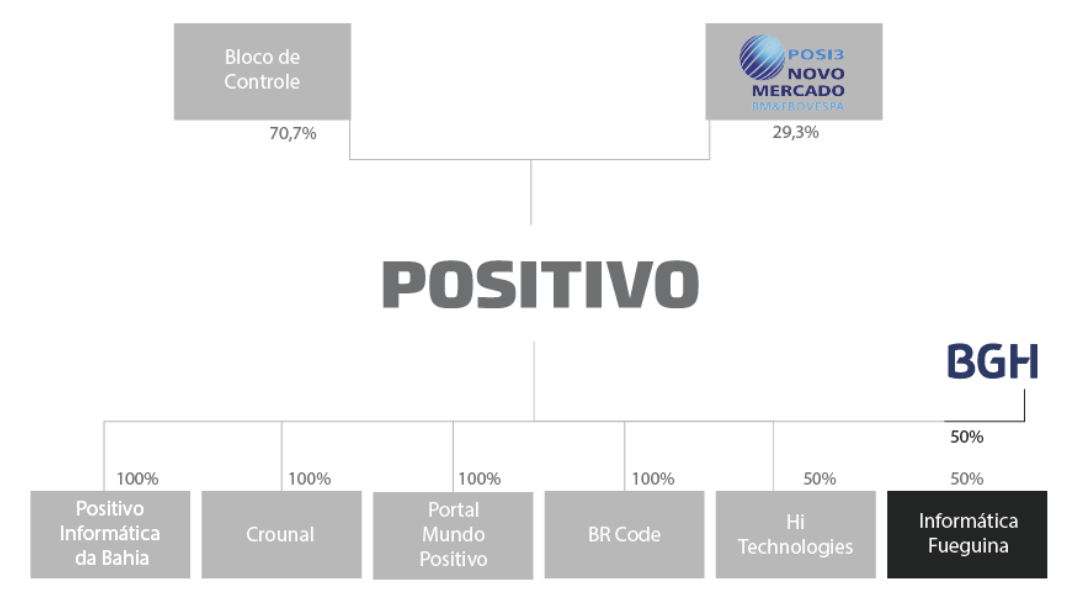
\includegraphics[width=1.0\textwidth]{Img/Corporativo}
\caption{Figura que demonstra o domínio e capital social da \nomeCompletoPositivo{}.}
\par\end{centering}
\end{figure}

Em 2016, a Positivo Tecnologia foi uma das maiores fabricantes de computadores no Brasil, respondendo por 15,3\% do número total de computadores vendidos no mercado brasileiro, de acordo com a IDC. No mesmo período, obtiveram uma participação de 19,9\% do mercado de varejo. Uma parcela substancial da produção de computadores é vendida através de grandes redes de varejo, com as quais o grupo mantém sólido relacionamento comercial, em função principalmente dos preços competitivos, do reconhecimento da marca e assistência técnica.

Adicionalmente, a companhia atua no mercado argentino por meio da marca \nomePositivoAr{}, fruto de uma joint venture com um parceiro local. Em 2015, os computadores \nomePositivoAr{} atingiram uma participação de 9,5\%, segundo a IDC.

No Brasil, a Positivo Tecnologia oferece uma linha completa de dispositivos, incluindo computadores de mesa (desktops e all-in-ones), computadores portáteis (notebooks e netbooks) e tablets, que são produzidos em Manaus (AM). Em 2012, a Companhia ingressou no mercado de telefones celulares, com a oferta de smartphones e messaging phones.

\begin{figure}[h]
\begin{centering}
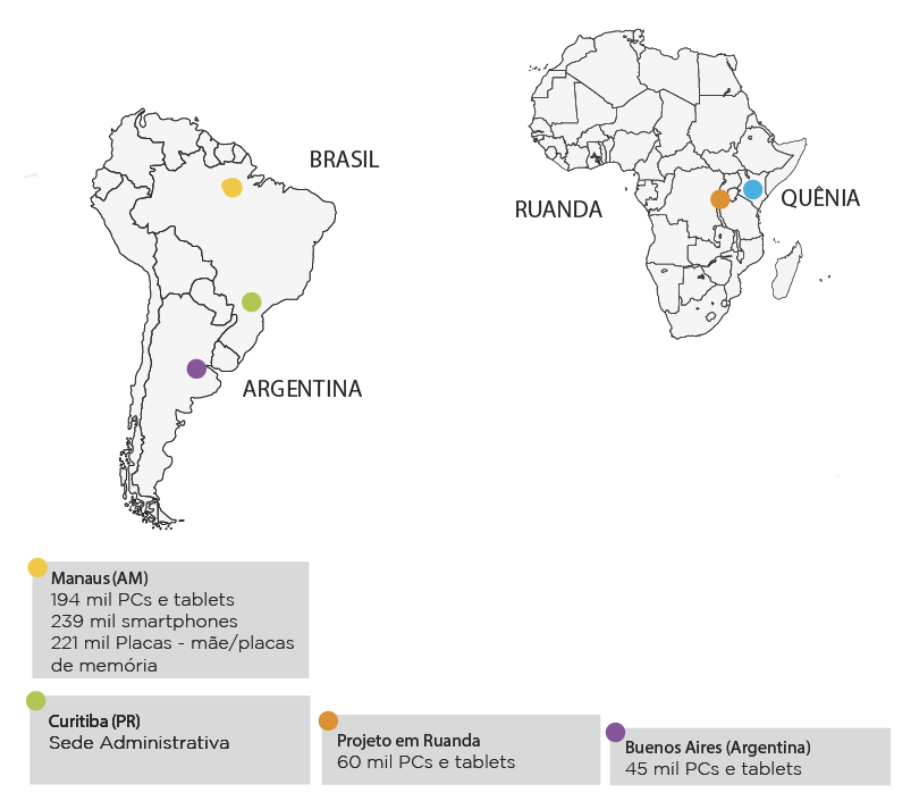
\includegraphics[width=1.0\textwidth]{Img/PositivoMundo}
\caption{Operações da \nomePositivo{} a nível mundial, bastante expressiva na América Latina e observa-se também sítios na África.}
\par\end{centering}
\end{figure}

Além disso, para atendimento e suporte aos milhões de consumidores finais, empresas e órgãos do governo, conta com uma ampla e capacitada rede de assistências técnicas cobrindo a totalidade do território nacional, e com a CRP - Central de Relacionamento Positivo, que registrou em média, 2,9 mil contatos diários em 2016. Grande parte destes contatos se refere a questões básicas sobre uso do computador, sistema operacional ou problemas com conexões, uma vez que muitos dos clientes estão adquirindo seu computador pela primeira vez.

Parcela menor da receita da Companhia provém do Segmento de Tecnologia Educacional, no qual acredita ser líder absoluto no País. A Companhia oferece soluções de infraestrutura e gestão, aplicativos e plataformas educacionais, portais de educação, além de formação de professores e acompanhamento pedagógico. Os portais têm mais de 1,2 milhões de usuários ativos, com modelo de receita recorrente mensal. 

As soluções educacionais da Positivo Tecnologia estão presentes em mais de 14 mil escolas e são exportadas para mais de 40 países. Dentre os principais produtos estão mesas educacionais, dispositivos móveis, lousas interativas, dispositivos de armazenamento e recarga, projetores, acess point, e sistema de gerenciamento de aulas. A Companhia é também distribuidor exclusivo no Brasil de empresas líderes no desenvolvimento e distribuição de software educacional, bem como distribui produtos da LEGO\texttrademark Education no território nacional.

Em 2016, a Companhia ingressou no mercado de tecnologia médica por meio da aquisição de 50\% do capital social da Hi Technologies S.A., empresa com forte foco em P\&D para a oferta de produtos inovadores em saúde.


\chapter[Análise de Macroambiente]{Análise de Macroambiente}
\label{chap:macro}
Para tomar-se a decisão de investimento, deve-se considerar cuidadosamente todas as informações disponíveis sobre a Companhia, em especial os riscos levantados.

Os negócios, situação financeira e resultados de operações da Positivo Tecnologia podem ser adversa e materialmente afetados por quaisquer desses riscos e, por conseguinte, impactar negativamente os títulos emitidos pela Companhia.

Os riscos descritos neste capítulo são os mais relevantes referentes a companhia. Os demais riscos, não identificados aqui ou pela própria Positivo Tecnologia, podem ainda assim afetar os seus negócios.

\section{Riscos Relacionados ao Setor}

\subsection{Variação do Dólar} A maioria das matérias-primas e/ou componentes utilizados são importados ou têm seus preços diretamente atrelados ao dólar americano, de forma que uma oscilação brusca e/ou inesperada poderá ter um efeito adverso relevante. Assim, é necessário repassar parte da flutuação cambial nos preços dos produtos finais. Como nem sempre é possível repassar-se esse valor aos clientes, pode haver perda expressiva na margem de lucro dos produtos afetados.

Uma mudança drástica na flutuação cambial implica também em necessidade de aumento do preço final do produto, que é especializado nas classes B e C e por isso podem diminuir de maneira significativa o volume de vendas da empresa.

\subsection{Benefícios Fiscais} 
A Companhia é titular de benefícios fiscais federais e estaduais concedidos para a indústria de computadores e a suspensão. O cancelamento ou a não renovação de tais benefícios podem afetar adversamente os resultados da Companhia, tais benefícios lhe garante redução nas alíquotas de IPI e isenção das alíquotas das contribuições ao PIS/PASEP e COFINS incidentes sobre a receita bruta proveniente de vendas diretas ao consumidor final de desktops e de notebooks com preço máximo de R\$ 4.000 e de tablets com preço máximo de R\$ 2.500,00.

É também beneficiada pela subvenção para investimentos, proveniente da redução de ICMS promovida pelo Estado do Paraná, a qual permite crédito e redução de alíquota para 0\% sobre a venda de PCs. Caso a empresa deixe de cumprir determinadas obrigações a que está sujeita por força das normas e dos documentos que instrumentalizam a concessão de tais benefícios fiscais, seus benefícios poderão ser suspensos ou cancelados e a Companhia poderá ser obrigada a pagar integralmente o valor dos tributos devidos, acrescidos de encargos. Ademais, não é possível assegurar que, após o término de seu prazo de vigência, os benefícios fiscais de que atualmente a companhia é titular serão renovados ou, ainda, que esta conseguirá obter novos benefícios fiscais em condições favoráveis. 

\subsection{Interrupções na recomposição dos estoques}
Está sujeita a possíveis atrasos motivados por greves nas alfândegas, portos, aeroportos e receita, haja visto que boa parte das matérias primas e/ou componentes utilizados são importados. Haveria então atraso na entregas desses materiais pelos seus fornecedores, e, por consequência, sua capacidade produtiva. O mesmo vale para falhas na logística e transporte de matéria prima.

\subsection{Concorrência} 
Atua em segmentos de alta concorrência, tendo como competidores desde pequenas empresas a grandes multinacionais, enfrenta uma forte competição de um grupo concentrado de concorrentes locais e internacionais. No varejo, maior volume de vendas da Companhia, os principais concorrentes no segmento de desktops são empresas pertencentes a grupos nacionais, enquanto que no segmento de notebooks a empresa enfrenta principalmente a concorrência de grupos multinacionais, de presença global, com acesso ao mercado financeiro e de capitais a custos menores e prazos maiores.

\subsection{Mercado cinza (informal)}
Enfrenta também a concorrência de pequenos produtores locais que possuem boa aceitação em certos mercados, sendo que alguns deles operam no mercado cinza e, oferecendo preços mais baixos que os seus, o que pode vir a resultar na redução de seus preços e diminuição de suas vendas e margens. Também, novos concorrentes poderão entrar nos mercados em que atua e a participação de mercado da Companhia poderá ser reduzida caso esta não consiga se manter competitiva, principalmente no que se refere à manutenção dos preços de seus produtos ou serviços compatíveis com os orçamentos de seus clientes.

\subsection{Governo} 
A \nomePositivo{} é beneficiada por diversos programas governamentais que prevêem incentivos para a produção e a aquisição de PCs, como redução de alíquotas de impostos incidentes sobre a produção e a venda de PCs, como a MP do Bem e a Lei de Informática, que promovem a redução da alíquota de PIS/COFINS e de IPI, bem como a concessão de financiamentos atrativos para consumidores através do programa "Computador para Todos", a aquisição de laboratórios de informática para escolas públicas pelo MEC (Ministério da Educação) e de laboratórios de inclusão digital pelo MINICOM (Ministério das Comunicações), entre outros programas em esferas estaduais para incentivo à aquisição de PCs por parte de professores da rede pública de ensino, contudo, não pode garantir que futuros governos tenham a questão da inclusão digital da população nacional como prioridade.

Essas condições fiscais estão atreladas ao cenário político nacional e por isso há sempre o risco de serem revistas em determinado governo.

\section{Riscos Relacionados aos Negócios}

\subsection{Atrasos e descumprimentos de seus fornecedores} 
Tanto a sua produção como as suas receitas podem ser prejudicadas em razão de atrasos e descumprimentos de seus fornecedores, uma vez que a atividade se caracteriza pela manutenção de um nível de estoque adequado para suprir as necessidades de suas operações.  Tendo em vista a característica da indústria de componentes mundial, cuja produção é concentrada em poucos players, a Companhia tem poucos fornecedores, o que concentra o risco.

\subsection{Concentração das vendas} 
Parcela significativa das vendas está concentrada em grandes redes de varejo, essa  concentração em poucas grandes empresas aumenta seu poder de negociação nas regiões em que atuam e, consequesubsection{ente, essas empresas podem utilizar o seu poder de mercado para forçar a redução dos preços praticados pelas empresas do setor, o que pode ter um efeito adverso. No passado recente, foram realizadas algumas operações societárias entre empresas do setor varejista que aumentaram ainda mais essa concentração do mercado de varejo e elevando sua dependência.

\subsection{Interesse público}
A Positivo Tecnologia está sujeita a sanções impostas por descumprimento de contratos firmados com a administração pública em geral, bem como à rescisão unilateral de tais contratos em virtude de razões de interesse público, o que poderia afetar negativamente sua capacidade de participar em outras licitações públicas e/ou ter um efeito adverso, podendo afetar a marca da Companhia, seu resultado operacional e financeiro e seu fluxo de caixa, além de vir a impactar negativamente sua lucratividade por um período. Os prazos de recebimento de clientes de governo são usualmente superiores aos praticados nos mercados de varejo e corporativo, sendo que um crescimento nas vendas para este segmento poderia acarretar em maior necessidade de capital de giro, resultando em maior exposição do fluxo de caixa da Companhia.

\subsection{Exposição e reputação}
Está sujeita a reclamações de consumidores e defeitos de produtos, o que poderia afetar negativamente sua imagem e ter um efeito adverso. Caso a Companhia venha a ser responsabilizada ou condenada por defeitos, erros ou falhas de seus produtos em uma ação judicial, tal decisão poderá ter um efeito material adverso em seu negócio, sua marca, seu resultado operacional e financeiro e em seu fluxo de caixa, além de vir a impactar negativamente sua lucratividade.

\section{Riscos Relacionados à Companhia}

\subsection{Implementação de suas estratégias de negócio}
A Companhia pode não conseguir implementar integralmente suas estratégias de negócios. Como parte de sua estratégia de crescimento, procura potencializar continuamente a força da sua marca e busca o melhor posicionamento de suas marcas secundárias no mercado de varejo, bem como expandir seu volume de vendas e elevar seu desempenho operacional. Cas não seja capaz de implementar satisfatoriamente tais estratégias, terá como consequência, a diminuição de sua taxa de crescimento e de seus resultados operacionais. Não é possível assegurar que a capacidade de gerenciamento de crescimento será bem sucedida. 

\subsection{Capacidade de inovação}
Caso não seja capaz de introduzir produtos inovadores e tecnologicamente avançados em uma indústria caracterizada pela rápida obsolescência dos produtos, seu crescimento e seus esforços de manter sua lucratividade poderão ser afetados. Seu modelo de negócios depende de sua capacidade de introduzir de forma ágil produtos com tecnologia e design adequados aos anseios de seus consumidores, para que seja bem sucedida, depende de diversos fatores, tais como a disponibilidade de novos produtos, controle de qualidade eficaz, rapidez de seus esforços para o lançamento de produtos, acesso a fornecedores de tecnologia, correta estimativa da demanda, treinamento de seu pessoal de vendas e a aceitação, pelos consumidores, de novas tecnologias e designs. 

\subsection{Falhas sistêmicas e assistência técnica} 
A Companhia pode não conseguir identificar uma falha sistêmica durante o processo produtivo, podendo prejudicar a qualidade de seus produtos e, consequesubsection{ente, acarretar no aumento das despesas com assistência técnica. Seu modelo de gestão da qualidade inclui, na introdução de produtos e novos componentes, as etapas de qualificação de fornecedores, homologação de componentes, inspeção de recebimento, produção de lote piloto, testes funcionais durante a fase de produção e auditoria final de produto. Apesar destas etapas de controle, podem ocorrer falhas no processo de montagem ou no recebimento de um lote de componentes defeituoso, que só venham a ter seu efeito percebido durante a vida útil do produto. 

Caso não seja capaz de detectar a elevação do índice de falhas do parque em garantia e definir ações de contingência a fim de mitigar esses efeitos, o índice de falhas do parque em garantia em patamar superior ao índice previsto pode trazer como consequência um desabastecimento de peças para suprir os chamados de garantia, acarretando em atrasos no atendimento ao cliente, elevação dos custos com assistência técnica e consequesubsection{ente um elevado índice de reclamações em entidades judiciais, como por exemplo o Procon, o que poderia inclusive afetar negativamente a imagem.

\subsection{Seguros} 
Os seguros de que a Companhia é beneficiária podem não prover a cobertura completa dos riscos a que está sujeita, ou podem não estar disponíveis a um custo razoável. A ocorrência de perdas ou demais responsabilidades que não estejam cobertas por seguro, ou que excedam os limites dos seguros dos quais é beneficiária, poderão acarretar significativos custos adicionais não previstos, o que poderá ter um efeito adverso.

\subsection{Perda de Talentos}
O desligamento ou perda dos serviços de pessoas estratégicas ou sua inabilidade de atrair e manter outras pessoas estratégicas, pode afetar adversamente os seus negócios. Seu sucesso e crescimento futuro depende de sua habilidade em identificar, atrair e manter em seus quadros funcionários e administradores qualificados para ocupar posições estratégicas em sua estrutura e orientar vários aspectos da condução de seus negócios, como o mercado em que atua é muito competitivo, não é possível assegurar que esta terá sucesso.

\subsection{Controles Internos}
Com a perda dos serviços ou o falecimento de qualquer destes administradores, a Companhia poderá ser incapaz de implementar e manter controles internos de contabilidade, o que poderia causar a perda de confiança por parte de investidores em suas informações financeiras e um impacto adverso no preço de suas ações ordinárias. Vale ressaltar que no passado, foram identificadas deficiências nos seus controles internos de contabilidade, decorrentes principalmente de falhas na comunicação interna entre determinadas áreas da empresa. Essas deficiências, inicialmente, resultaram na emissão por seus auditores de pareceres com ressalvas às suas demonstrações financeiras para os anos de 2003 e 2004. 

Após a republicação pela Companhia das demonstrações para aqueles anos, essas ressalvas foram retiradas. Nos períodos seguintes, a Companhia documentou, testou e melhorou seus controles internos de contabilidade, sendo que suas demonstrações financeiras foram auditadas sem ressalvas. Mais adiante, ao final de 2009, foi implantado um Sistema Integrado de Gestão Empresarial, que trouxe significativas melhorias na eficiência operacional e qualidade dos seus controles, contudo, a ocorrência de uma falha como essa poderia afetar a confiança de investidores sobre suas demonstrações financeiras, e poderia causar um impacto adverso em seus resultados, posição financeira e no preço de suas ações ordinárias.

\subsection{Processos judiciais}
Decisões desfavoráveis em processos judiciais ou administrativos podem afetar adversamente seus negócios, condição financeira e resultados operacionais, não se pode assegurar que os resultados de processos judiciais em que é ré serão favoráveis ou considerados improcedentes, bem como que tais ações estejam plenamente provisionadas. A Companhia pode ter seus negócios, sua condição financeira e seus resultados operacionais adversamente afetados por decisões contrárias a seus interesses em ações que eventualmente alcancem valores substanciais ou que impeçam a realização de seus negócios conforme planejado.

\subsection{Riscos relacionados a operações no exterior}
Ao final de 2010, a Companhia constituiu um empreendimento em conjunto (joint venture) com a empresa argentina BGH Sociedad Anónima ("BGH"), que resultou na formalização da sociedade com controle compartilhado “Informática Fueguina S.A.”, que teve como objetivo fabricar e comercializar produtos de informática voltados aos mercados da Argentina e do Uruguai. A planta industrial está localizada na Província da Terra do Fogo, Antártida e Ilhas do Atlântico Sul, Argentina. Em função da natureza da operação, os principais riscos envolvem a administração compartilhada entre a Companhia e a BGH, a produção em localidade remota e a exploração de novos mercados. Dessa forma, os futuros resultados desta joint venture podem ser adversamente afetados por eventuais conflitos entre os sócios, dificuldades logísticas e aceitação dos produtos pelos consumidores locais. 

Adicionalmente, podem ocorrer eventuais restrições a remessas de divisas ao exterior, incluindo dividendos, além de dificuldades na importação de insumos em função da necessidade de autorizações prévias junto às autoridades locais, bem como dificuldades e penalidades relacionadas ao cumprimento de leis e regulamentações de governos estrangeiros.

Deve-se considerar também o enfrentamento de dificuldades relacionadas a condições competitivas adversas, instabilidade política e econômica, bem como riscos cambiais similares aos existentes na operação brasileira em função do descasamento entre moedas, uma vez que grande parte dos custos com insumos é atrelada ao dólar e os produtos são posteriormente comercializados em moeda local. Por meio de sua divisão de Tecnologia Educacional, a Companhia exporta mesas educacionais para países estrangeiros, operação que representa uma pequena parcela da receita do segmento de Tecnologia Educacional. 

\section{Riscos Relacionados aos Acionistas da Companhia}

\subsection{Conflito de interesses}
Os acionistas controladores poderão tomar medidas que podem ser contrárias aos interesses dos seus investidores, inclusive reorganizações societárias e condições de pagamento de dividendos, uma vez que detêm o controle efetivo, elegendo a maioria dos membros de seu Conselho de Administração. A decisão dos acionistas controladores quanto aos seus rumos pode divergir da decisão esperada por seus acionistas minoritários, porém nenhuma decisão será tomada pelos controladores em desacordo com a Lei, estatuto e regulamentação aplicável. A Companhia possui um membro independente em seu Conselho de Administração, de acordo com as normas do Novo Mercado da BMF\&BOVESPA.

\subsection{Necessidade de capital adicional}
A Companhia poderá ter interesse em captar recursos no mercado de capitais, por meio de emissão de ações e/ou colocação pública ou privada de títulos conversíveis em ações. A captação de recursos adicionais por meio da emissão pública de ações, que pode não prever direito de preferência aos acionistas, poderá acarretar diluição da participação acionária do investidor no seu capital social.

\subsection{Não pagamento de dividendos}
De acordo com seu Estatuto Social, a Companhia deverá pagar aos seus acionistas 25\% de seu lucro líquido anual sob a forma de dividendo obrigatório, contudo, como o lucro líquido pode ser capitalizado, utilizado para compensar prejuízo ou então retido, conforme previsto na Lei das Sociedades por Ações, este pode não ser disponibilizado para pagamento de dividendos.

\subsection{Disposições de limitação e controle}
O Estatuto Social da companhia contém disposições para evitar a concentração das ações da Companhia em pequeno grupo de investidores, de sorte a promover a dispersão das ações. Uma dessas disposições exige que qualquer acionista (que não aqueles que já sejam acionistas da Companhia no dia da publicação do anúncio de início de sua oferta pública inicial, e demais investidores que se tornem acionistas da Companhia em certas transações especificadas em seu Estatuto Social) que passe a deter 10\% ou mais do capital social da Companhia (excluindo-se ações em tesouraria e aumentos de capital involuntários, conforme especificado em seu Estatuto Social) realize oferta pública da totalidade das ações em circulação por preço estabelecido em conformidade com o Estatuto Social no prazo de 30 (trinta) dias contados da aquisição da aludida participação. Essas disposições podem resultar em desincentivo a que terceiros adquiram o controle da companhia em operações que assegurariam aos detentores de nossas ações o direito de vendê-las a tal terceiro (\emph{tag along}).

\section{Análise de Fatores PESTAL}

A análise PESTAL avalia as contribuições dos fatores \emph{políticos, econômicos, sociais, tecnológicos, ambientais e legais}.

\subsection{Políticos}
O cenário político atual apresenta correlação direta com o cenário econômico. Sendo assim, dependendo do desfecho da eleição presidencial, o panorama macro econômico pode se alterar de tal maneira que o país mergulhe em um longo período de crise. Dado que a empresa obtém seus resultados da venda de equipamentos de informática, majoritariamente no mercado B2B, caso o país mantenha-se em um cenário de desaquecimento econômico, empresas optarão por postergar a renovação de seus parques tecnológicos, impactando diretamente a Positivo.

\subsection{Econômicos}

Assim como o cenário político é influenciado pelo cenário econômico, o mesmo é influenciado pelo primeiro. Sendo assim, conforme citado acima, um dos riscos econômicos a operação do Grupo Positivo é a revogação de isenções tributárias relacionadas a produção dos produtos de tecnologia do grupo. Outro ponto que deve ser ressaltado é a dependência matéria prima e componentes internacionais que possuem seus preços lastreados em dólar. Uma variação desfavorável do câmbio da moeda em relação ao real irá impactar as margens de lucro do grupo, sendo que, no limite, pode prejudicar a saúde financeira da empresa. Por último a estruturação das dívidas da empresa poderá sofrer um impacto significativo caso o governo altere a política de juros.
%A Positivo é influenciada positivamente por uma cotação favorável do dólar, uma vez que seu maior fornecedor, a \emph{BGH} atua na América Latina (Argentina). A estabilização e melhora progressiva do cenário nacional brasileiro desde a crise de 2013 tem também aquecido as vendas na empresa, havendo um aumento significativo tanto nas vendas ao varejo quanto ao mercado B2B. As taxas de juros mais favoráveis, afetam também diretamente o endividamento da empresa, e portanto, a atual conjectura econômica tem impacto favorável as operações interancionais da empresa.

\subsection{Sociais}
A tendência social em relação a computadores pessoais é de declínio. Poucas pessoas optam por ter um desktop em casa, o mesmo vem acontecendo com laptop. Com o aumento da capacidade dos celulares e tablets, computadores pessoais estão perdendo mercado. Sendo assim, é necessário que a Positivo se adeque a esta nova tendência, movimento que já pode ser percebido com a linha Quantum de celulares smartphone.

\subsection{Tecnológicos}
O paradigma tecnológico esta prestes a sofrer uma nova ruptura. Nos anos 2000, os smartphones mudaram a maneira como o ser humano via tecnologia. A simplicidade que o smartphone trouxe aos seus usuários expandiu o mercado de tecnologia enormemente. Agora, próximos aos anos 2020, estamos na beira de uma nova revolução. Realidade aumentada, impressoras 3D e computação em nuvem promsubsection{ mudar os modelos de negócios de empresas de tecnologia. Não será mais necessária alta capacidade de processamento embarcada. Os gadgets irão mudar de forma e função. É uma ameaça a qualquer empresa essa mudança de paradigma. Apenas os que forem ágeis irão perdurar e prosperar.

\subsection{Ambientais}
Ano a ano a legislação ambiental ao redor do mundo torna-se mais restritiva. Além disso, a consciência ambiental da população vem pressionando empresas e governos a tomarem posições mais responsáveis sobre os meios de produção e geração de resíduos. Isso não é diferente para a indústria de eletroeletrônicos, a qual a Positivo esta inserida. Desde 2010, existe uma pressão crescente e constante em relação a responsabilidade empresarial no tocante aos resíduos de manufatura e descarte de equipamentos obsoletos. Nos países europeus, já é realidade a obrigação das empresas em relação a logística reversa de equipamentos obsoletos, além do descarte adequado de resíduos. No Brasil, ainda engatinhamos nestes temas, porém, inevitavelmente estes terão de ser abordados seriamente. Dada a multiplicidade de aparelhos portados por cada indivíduo, a logística reversa e posterior destinação adequada dos mesmos tornar-se-á um desafio a ser superado.

\subsection{Legais}
No âmbito legal, existe a eterna promessa governamental de simplificação redução de tributos. Simplificações de cobrança de tributos iriam beneficiar enormemente o setor de eletroeletrônicos, que devido à complexidade e a infinidade de componentes presentes em cada aparelho, enfrentam um verdadeiro pesadelo fiscal na hora de atribuir e contabilizar os tributos referentes a cada aparelho. Caso a promessa de desoneração e simplificação tributária se concretize, a Positivo poderá expandir a sua penetração no mercado nacional e internacional, fornecendo produtos a um custo menor.

\section{Análise SWOT}

A análise SWOT é constitúida como uma matriz de fatores \emph{internos e externos} que são parte do ambiente de negócios da empresa. No caso da positivo, baseia-se as análises naquilo que está disponível no portal da empresa\cite{fatoresDeRisco2018}\cite{positivo2t18}.

\subsection{Fatores Externos}

\begin{center}
\begin{table}[H]
\begin{centering}
\begin{tabular}{>{\centering}p{0.55\textwidth}|>{\centering}p{0.4\textwidth}}
\hline 
Oportunidades & Ameaças\tabularnewline
\hline 
Capitalizar a posição de liderança para aproveitar o potencial de
crescimento do varejo. & Atuação em um setor que se caracteriza pela rápida obsolescência de
seus estoques.\tabularnewline
\hline 
Aumentar sua participação no setor corporativo criando estrutura para
atuar especificamente com PMEs que é um mercado que em 2016 representava
72\% do setor.  & Necessidade de alto nível de investimento em desenvolvimento e pesquisa
para que a empresa consiga manter seus produtos atrativos aos clientes.\tabularnewline
\hline 
Consolidar sua posição de vanguarda no lançamento de produtos adaptados
ao mercado brasileiro por meio de sua agilidade na adaptação de produtos
e no fornecimento de soluções integradas, mantendo também o fornecimento
de dispositivos aos segmentos de varejo, corporativo e governo, no
Brasil, Argentina, Uruguai, Chile, na América e Ruanda e Quênia, na
África. & Matérias primas e principais componentes são importados e tem seus
preços diretamente atrelados ao dólar. Oscilações cambiais relevantes
podem ter um forte impacto nas vendas e nos resultados da companhia.\tabularnewline
\hline 
Aproveitar oportunidades adicionais de crescimento do negócio direcionando
parte da obrigação de investimentos em pesquisa e desenvolvimento,
exigidos em contrapartida a benefícios fiscais, para oportunidades
lucrativas de crescimento no segmento Tecnologico Educacional.  & Aumento nas taxas de juros podem comprometer as vendas, uma vez que
as classes sociais focadas pela positivo poderão conter o seu consumo
em virtude de grande parte das aquisições efetuadas ser através do
crédito ao consumidor. \tabularnewline
\hline 
Focar em eficiência operacional e controle de custos instalando unidades
fabris em locais que ofereçam vantagens logísticas e fiscais.  & \tabularnewline
\hline 
Manter sua sólida posição financeira mantendo o baixo nível de endividamento
e fazendo hedge cambial de uma porção significativa de suas obrigações
em moeda estrangeira, com o objetivo de proporcionar estabilidade
contra oscilações macroeconômicas.  & \tabularnewline
\hline 
\end{tabular}
\par\end{centering}
\caption{Tabela de Oportunidades x Ameaças, parte da análise SWOT de fatores \emph{externos}}
\end{table}
\par\end{center}

\subsection {Fatores Internos}

\begin{center}
\begin{table}[H]
\begin{centering}
\begin{tabular}{>{\centering}p{0.55\textwidth}|>{\centering}p{0.4\textwidth}}
\hline
Forças & Fraquezas\tabularnewline
\hline
Líder de vendas de computadores no mercado brasileiro há mais de 10
anos consecutivos.  & Percentual considerável das vendas está concentrado em grandes redes
de varejo, que possuem estratégias agressivas de negociação e buscam
obter ganhos em relação a seus concorrentes.\tabularnewline
\hline
Forte relacionamento com grandes redes de varejo.  & \tabularnewline
\hline
Grande investimento na marca com ações de marketing e trade marketing
contando com uma equipe de 200 promotores próprios.  & \tabularnewline
\hline
Ampla rede de assistências técnicas.  & \tabularnewline
\hline
Custos reduzidos e preços competitivos com grande escala de fabricação
e acesso diretamente a grandes fornecedores mundiais.  & \tabularnewline
\hline
\end{tabular}
\par\end{centering}
\caption{Tabela de Forças x Fraquezas, parte da análise SWOT, para fatores
\emph{internos}}
\end{table}
\par\end{center}

\section{Análise das Cinco Forças de Porter}

\begin{table}[H]
\begin{tabular}{>{\centering}p{0.3\textwidth}|>{\centering}p{0.4\textwidth}|>{\centering}p{0.3\textwidth}}
\cline{2-2} 
 & \textbf{Novos Entrantes} & \tabularnewline
\cline{2-2} 
 & A maioria da matéria prima utilizada pela Positivo é importada, o
que a deixa refém de variações cambiais\cite{em2017}.  & \tabularnewline
\hline 
\multicolumn{1}{|>{\centering}p{0.3\textwidth}|}{\textbf{Fornecedores}} & \textbf{Concorrentes} & \multicolumn{1}{>{\centering}p{0.3\textwidth}|}{\textbf{Clientes}}\tabularnewline
\hline 
\multicolumn{1}{|>{\centering}p{0.3\textwidth}|}{O maior mercado da Positivo, é o de PC\textquoteright s, produto que
há tempo já stá sendo substituído por celulares e tablets, porém essa
substituição ainda levará tempo, principalmente no mercado corporativo
e a Positivo está cada vez mais ampliando sua participação em outros
mercados, como celulares, serviços médicos, etc. } & A Positivo não conta com grandes concorrentes brasileiros, porém conta
com vários concorrentes estrangeiros de peso como Lenovo, HP, Dell,
Acer, Samsung e Asus no mercado de PCs e Notebooks. E ainda conta
com uma esmagadora concorrência da Apple e Samsung na mercado de celulares.
A maior fonte de receita da Positivo são com computadores, o que representa
65\%. Ela lidera o mercado com 17,8\% de market share. No mercado
de celulares ela tem um share de 3\% incluindo os modelos mais simples.
Ao adquirir 50\% da Hi Technologies em 2016 ela passou a ser a primeira
empresa do mundo a fazer análises laboratoriais em minutos.  & \multicolumn{1}{>{\centering}p{0.3\textwidth}|}{A Positivo Tecnologia conta com grande variedade de clientes desde
o setor corporativo, varejo, educacional, governo e mais recente na
área da saúde. Além de ter uma participação de 9,5\% no mercado argentino
através da marca BGH. }\tabularnewline
\hline 
 & \textbf{Substitutos} & \tabularnewline
\cline{2-2} 
 & O maior mercado da Positivo, é o de PC\textquoteright s, produto que
há tempo já está sendo substituído por celulares e tablets, porém
essa substituição ainda levará tempo, principalmente no mercado corporativo
e a Positivo está cada vez mais ampliando sua participação em outros
mercados, como celulares, serviços médicos, etc\cite{analisandoAcoes2017}. & \tabularnewline
\cline{2-2} 
\end{tabular}

\caption{A tabela relaciona as cinco forças de Porter para a \nomePositivo.}
\end{table}


\chapter[Análise de Microambiente]{Análise de Microambiente}
\section{Interna}

\begin{itemize}
\item O canal de vendas passa por um momento de maior tensão entre fabricantes e redes varejistas, em função de negociações constantes para repasse da valorização do dólar.
\item Diminuição nas despesas com marketing devido à alta proporção de vendas no mercado de governo, que não consome estas verbas.
\item Aumento de assistência técnica decorrente do aumento no volume de vendas com maior prazo de garantia contratual para clientes de governo e corporativo.
\item A companhia praticou maiores descontos nas vendas de celulares para combater o acirramento do ambiente competitivo.
Recorrentes contratações de hedge no intuito de controlar a variação cambial e negociar a elevação de preço junto aos canais de venda.
\item Aumento no volume de vendas garantindo o avanço do market share da companhia, atingindo o maior patamar em dois anos.
Rodada de captação de investimentos pela sociedade investida Hi Technologies S.A. afim de proporcionar maior robustez financeira para suportar sua expansão, além de facilitar futuras rodadas de captação no exterior.
\item Terceira vez consecutiva, as marcas Positivo e Quantum, da Positivo Tecnologia, são indicadas entre as empresas com melhor atendimento do Brasil, pelo prêmio Época Reclame Aqui.
Expectativa de maior faturamento com smartphones integrados a terminais de pagamento de débito e crédito.

\end{itemize}

\section{Externa}
\subsection{Mercado de Computadores}
\begin{itemize}
\item Expansão nas vendas de PC mesmo em um período impactado por eventos como a greve nacional dos caminhoneiros, a valorização expressiva do dólar e a copa do mundo.
\item Maior dificuldade na aquisição de insumos como memórias e SSDs, cujos preços no mercado internacional aumentaram significativamente.
\item Redução pontual nas entregas e vendas em função das eleições, com retomada das vendas após este período.
\end{itemize}

\subsection{Mercado de Telefones Celulares}
\begin {itemize}
\item Forte competição entre as marcas líderes.
\item Limitação de espaço para os demais competidores, resultando em queda de vendas para a maioria destas empresas.
\end{itemize}


\chapter[Análise de Demonstrações Financeiras]{Análise de Demonstrações Financeiras}
A análise de de demonstrações financeiras é composta pelas análises \emph{horizontal}, \emph{vertical} e \emph{por meio de índices}, as quais embasam a demonstração financeira da companhia em questão.

\section{Análise Horizontal}

\textcolor{blue}{A FAZER}

\section{Análise Vertical}

\textcolor{blue}{A FAZER}

\section{Análise por Meio de Índices}

\textcolor{blue}{A FAZER}


\chapter[Conclusão]{Conclusão}
\label{chap:conclusao}

\begin{figure}
\begin{centering}
\subfloat[\label{fig:prototipo-familia}Conforto,
espaço e filhos.]{\begin{centering}
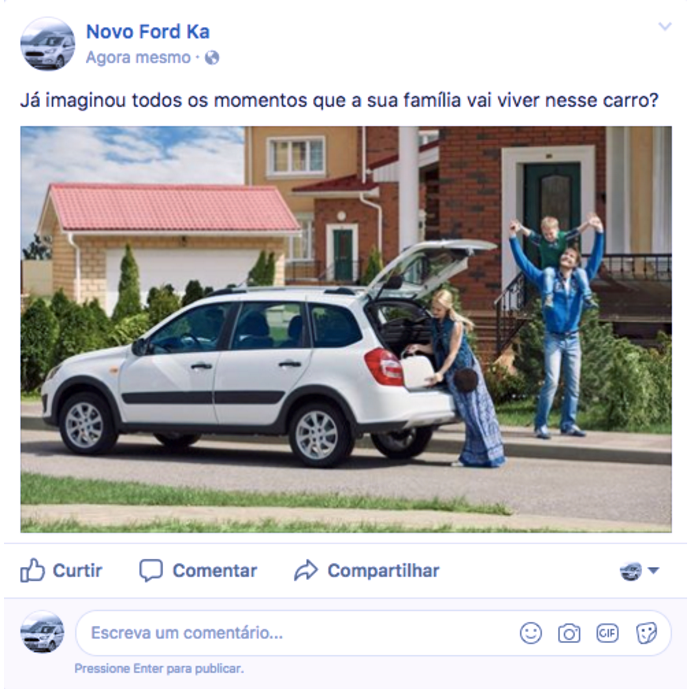
\includegraphics[height=0.30\textheight]{Imagens/p1_familia}~~
\par\end{centering}
}\subfloat[\label{fig:prototipo-versatil}Aborda o efeito versátil do carro.]{\begin{centering}
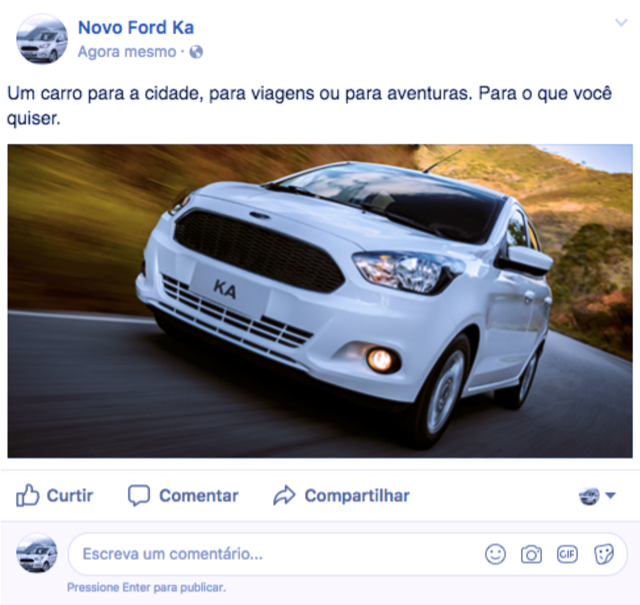
\includegraphics[height=0.30\textheight]{Imagens/p1_prototipo}
\par\end{centering}
}
\par\end{centering}
\caption{Peças ilustrativas de uma campanha em formato carrossel.}
\end{figure}

De acordo com o desenvolvido no capítulo \ref{chap:analise}, com
as tabelas \ref{tab:prototipo-vs-cluster} e \ref{tab:prototipo-analise},
contrasta a homogeneidade dos protótipo 2 e 3 à heterogeneidade do
protótipo 1. À primeira vista, percebe-se que os três protótipos possuem
proporções da população muito parecidas, entretanto há uma grande
diferença entre o protótipo 1, heterogêneo, com os demais protótipos.
Isto é, a possibilidade de uma campanha publicitária informativa unida
a transformativas que possibilitarão, se escolhido o protótipo 1,
abranger também os clusters \nomeCc{} e \nomeCb{}, dado que pela
própria heterogeneidade do protótipo 1, certas propagandas que apelam
para determinadas características do protótipo podem aumentar a aceitação
de uma campanha baseada neste protótipo.

\begin{table}
\begin{centering}
\begin{tabular}{c|>{\centering}p{0.28\textwidth}|>{\centering}p{0.28\textwidth}|>{\centering}p{0.28\textwidth}}
\hline 
 & Protótipo 1 & Protótipo 2 & Protótipo 3\tabularnewline
\hline 
Bom & Preferido entre \nomeCa{} e \nomeCd{}. & Amplamente preferido pelo cluster dos \nomeCc{}. & Amplamente preferido pelos \nomeCb{}, focados em Imagem.\tabularnewline
\hline 
Ruim & Somente uma estratégia de marketing não é suficiente, dada a sua heterogeneidade
e várias afinidades. & Difícil para a publicidade porque se mostra indiferente a carros.
Importam-se apenas com o preço. & Uma campanha publicitária em Imagem somente não gera interesse de
outros clusters.\tabularnewline
\hline 
\end{tabular}
\par\end{centering}
\caption{\label{tab:prototipo-analise}Vantagens e desvantagens por protótipos.}
\end{table}


Por exemplo, se uma campanha publicitária apelar de maneira informativa
e transformativa para os aspectos de Imagem e Utilitário do carro,
é possível abranger os clusters mencionados anteriormente, sustentando
assim uma aceitação maior por parte da população. Ou seja, escolhe-se
a versatilidade do protótipo 1, numa eventual campanha publicitária
como elemento.

\begin{figure}
\begin{centering}
\subfloat[\label{fig:painel-cambio}Acabamento e câmbio.]{\begin{centering}
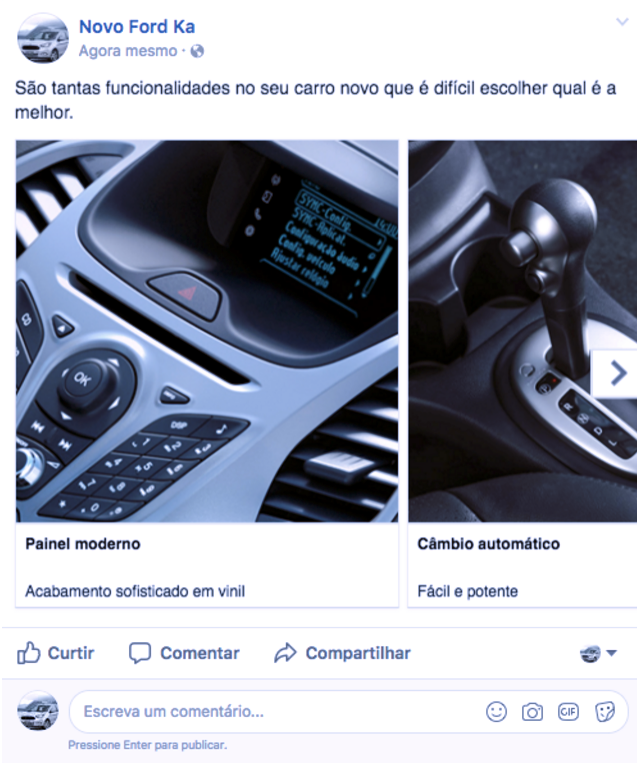
\includegraphics[height=0.34\textheight]{Imagens/p1_interior}
\par\end{centering}
}~~\subfloat[\label{fig:ar}Ar-condicionado.]{\begin{centering}
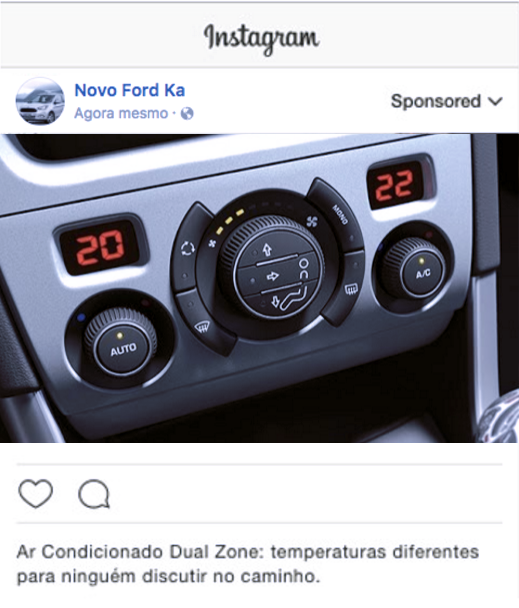
\includegraphics[height=0.34\textheight]{Imagens/p1_interior_painel}
\par\end{centering}
}
\par\end{centering}
\caption{Peças multifuncionais para Utilitário e Imagem.}
\end{figure}


\section{Recomendações para Campanha Publicitária}

Com base nas características analisadas dos grupos \nomeCa{} e \nomeCd{}
será feita uma combinação de campanhas publicitárias: para os \nomeCa{},
uma campanha transformativa mesclando os três atributos: Imagem, Utilitário
e Preço. Para os \nomeCd{}, uma campanha ressaltando o carro como
utilitário. Por se tratar de dois grupos diferentes vamos destacar
multifuncionalidade, tecnologia, versatilidade e conforto.

É possível uma campanh que foque nas seguintes características: confortável
e espaçoso. O público-alvo seriam os \nomeCd{} que preferem carros
como bens utilitários, destacando o porta-malas espaçoso para a família.
Os \nomeCd{} são formados predominantemente por mulheres com filhos,
por isso o destaque a família, na figura \ref{fig:prototipo-familia}.

A campanha com formato em carrossel irá abordar a característica de
multifuncionalidade. A publicidade tem foco nos \nomeCa{} combinando
funcionalidades (Utilitário) que valorizem o carro (Preço) e que tragam
mais sofisticação (Imagem), como vê-se nas figuras \ref{fig:painel-cambio}
e \ref{fig:ar}.

Finalmente, a figura \ref{fig:prototipo-versatil} seria veiculada
em formato vídeo, tanto em Facebook quanto na televisão. Destaca a
versatilidade do Ford Ka\texttrademark, valorizando o fato de ser
um carro potente (Utilitário) e ainda assim econômico (Preço). Em
televisão, dá-se preferência é por intervalos de jogos de futebol
buscando atingir um público predominantemente masculino que gosta
de esportes e aventuras. 



% ----------------------------------------------------------
% Finaliza a parte no bookmark do PDF
% para que se inicie o bookmark na raiz
% e adiciona espaço de parte no Sumário
% ----------------------------------------------------------
\phantompart

% ---
% Conclusão - Recomendação de qual protótipo
% ---
%\chapter{Conclusões}
% ---

%Placeholder
%\label{chap:conclusao}

\begin{figure}
\begin{centering}
\subfloat[\label{fig:prototipo-familia}Conforto,
espaço e filhos.]{\begin{centering}
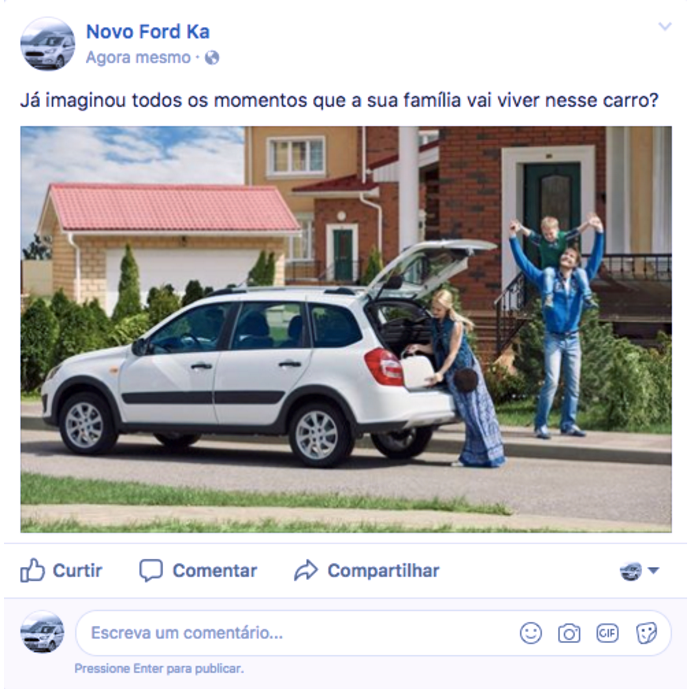
\includegraphics[height=0.30\textheight]{Imagens/p1_familia}~~
\par\end{centering}
}\subfloat[\label{fig:prototipo-versatil}Aborda o efeito versátil do carro.]{\begin{centering}
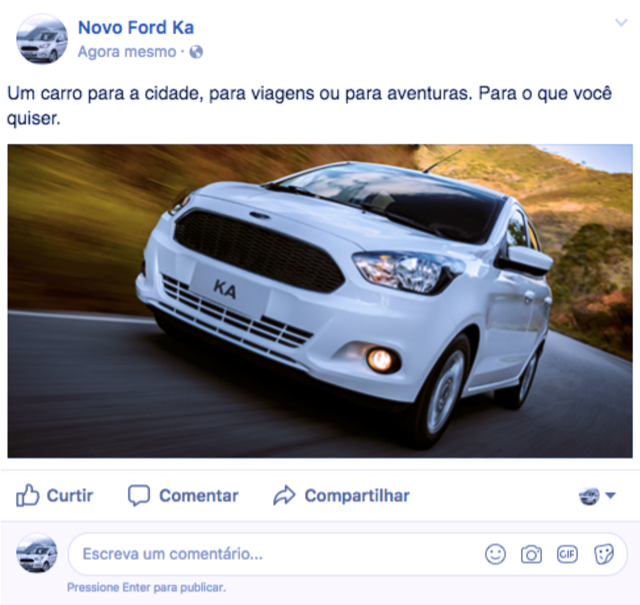
\includegraphics[height=0.30\textheight]{Imagens/p1_prototipo}
\par\end{centering}
}
\par\end{centering}
\caption{Peças ilustrativas de uma campanha em formato carrossel.}
\end{figure}

De acordo com o desenvolvido no capítulo \ref{chap:analise}, com
as tabelas \ref{tab:prototipo-vs-cluster} e \ref{tab:prototipo-analise},
contrasta a homogeneidade dos protótipo 2 e 3 à heterogeneidade do
protótipo 1. À primeira vista, percebe-se que os três protótipos possuem
proporções da população muito parecidas, entretanto há uma grande
diferença entre o protótipo 1, heterogêneo, com os demais protótipos.
Isto é, a possibilidade de uma campanha publicitária informativa unida
a transformativas que possibilitarão, se escolhido o protótipo 1,
abranger também os clusters \nomeCc{} e \nomeCb{}, dado que pela
própria heterogeneidade do protótipo 1, certas propagandas que apelam
para determinadas características do protótipo podem aumentar a aceitação
de uma campanha baseada neste protótipo.

\begin{table}
\begin{centering}
\begin{tabular}{c|>{\centering}p{0.28\textwidth}|>{\centering}p{0.28\textwidth}|>{\centering}p{0.28\textwidth}}
\hline 
 & Protótipo 1 & Protótipo 2 & Protótipo 3\tabularnewline
\hline 
Bom & Preferido entre \nomeCa{} e \nomeCd{}. & Amplamente preferido pelo cluster dos \nomeCc{}. & Amplamente preferido pelos \nomeCb{}, focados em Imagem.\tabularnewline
\hline 
Ruim & Somente uma estratégia de marketing não é suficiente, dada a sua heterogeneidade
e várias afinidades. & Difícil para a publicidade porque se mostra indiferente a carros.
Importam-se apenas com o preço. & Uma campanha publicitária em Imagem somente não gera interesse de
outros clusters.\tabularnewline
\hline 
\end{tabular}
\par\end{centering}
\caption{\label{tab:prototipo-analise}Vantagens e desvantagens por protótipos.}
\end{table}


Por exemplo, se uma campanha publicitária apelar de maneira informativa
e transformativa para os aspectos de Imagem e Utilitário do carro,
é possível abranger os clusters mencionados anteriormente, sustentando
assim uma aceitação maior por parte da população. Ou seja, escolhe-se
a versatilidade do protótipo 1, numa eventual campanha publicitária
como elemento.

\begin{figure}
\begin{centering}
\subfloat[\label{fig:painel-cambio}Acabamento e câmbio.]{\begin{centering}
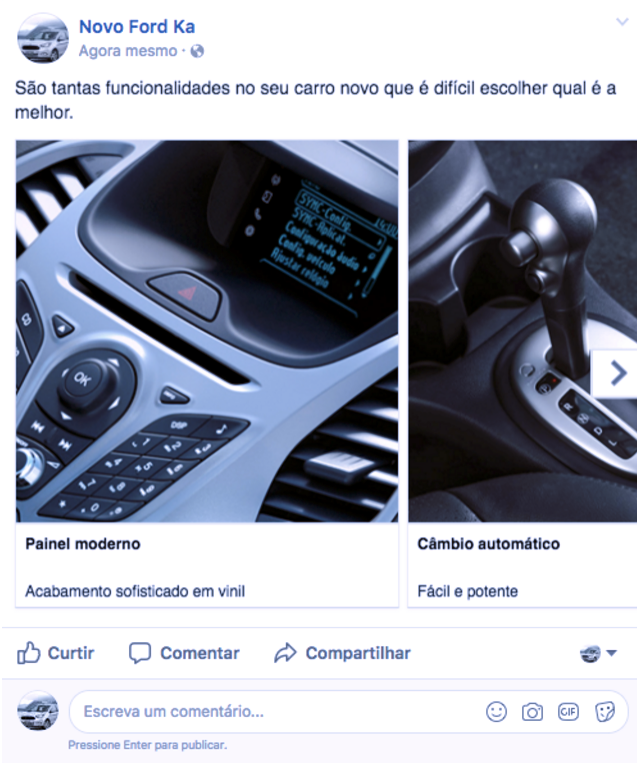
\includegraphics[height=0.34\textheight]{Imagens/p1_interior}
\par\end{centering}
}~~\subfloat[\label{fig:ar}Ar-condicionado.]{\begin{centering}
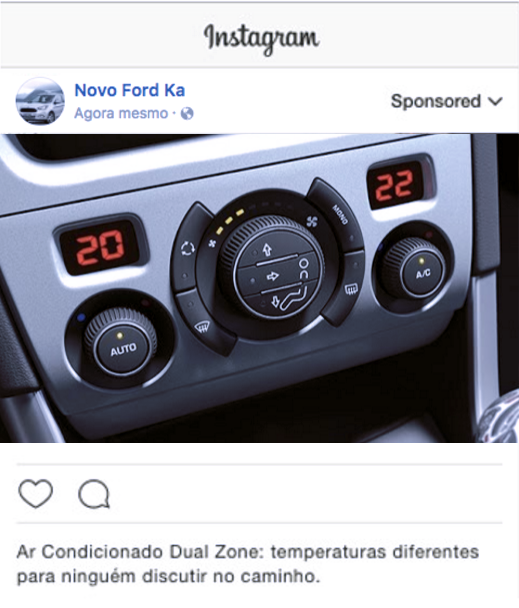
\includegraphics[height=0.34\textheight]{Imagens/p1_interior_painel}
\par\end{centering}
}
\par\end{centering}
\caption{Peças multifuncionais para Utilitário e Imagem.}
\end{figure}


\section{Recomendações para Campanha Publicitária}

Com base nas características analisadas dos grupos \nomeCa{} e \nomeCd{}
será feita uma combinação de campanhas publicitárias: para os \nomeCa{},
uma campanha transformativa mesclando os três atributos: Imagem, Utilitário
e Preço. Para os \nomeCd{}, uma campanha ressaltando o carro como
utilitário. Por se tratar de dois grupos diferentes vamos destacar
multifuncionalidade, tecnologia, versatilidade e conforto.

É possível uma campanh que foque nas seguintes características: confortável
e espaçoso. O público-alvo seriam os \nomeCd{} que preferem carros
como bens utilitários, destacando o porta-malas espaçoso para a família.
Os \nomeCd{} são formados predominantemente por mulheres com filhos,
por isso o destaque a família, na figura \ref{fig:prototipo-familia}.

A campanha com formato em carrossel irá abordar a característica de
multifuncionalidade. A publicidade tem foco nos \nomeCa{} combinando
funcionalidades (Utilitário) que valorizem o carro (Preço) e que tragam
mais sofisticação (Imagem), como vê-se nas figuras \ref{fig:painel-cambio}
e \ref{fig:ar}.

Finalmente, a figura \ref{fig:prototipo-versatil} seria veiculada
em formato vídeo, tanto em Facebook quanto na televisão. Destaca a
versatilidade do Ford Ka\texttrademark, valorizando o fato de ser
um carro potente (Utilitário) e ainda assim econômico (Preço). Em
televisão, dá-se preferência é por intervalos de jogos de futebol
buscando atingir um público predominantemente masculino que gosta
de esportes e aventuras. 



% ----------------------------------------------------------
% ELEMENTOS PÓS-TEXTUAIS
% ----------------------------------------------------------
\postextual
% ----------------------------------------------------------

% ----------------------------------------------------------
% Referências bibliográficas
% ----------------------------------------------------------
\bibliography{referencias}

% ----------------------------------------------------------
% Glossário
% ----------------------------------------------------------
%
% Consulte o manual da classe abntex2 para orientações sobre o glossário.
%
%\glossary

% ----------------------------------------------------------
% Apêndices
% ----------------------------------------------------------

% ---
% Inicia os apêndices
% ---
\begin{apendicesenv}

%% Imprime uma página indicando o início dos apêndices
\partapendices

%% ----------------------------------------------------------
%\chapter{Quisque libero justo}
%% ----------------------------------------------------------

%\lipsum[50]

\chapter[Demonstrativos Financeiros]{Demonstrativos Financeiros}
\vspace*{-60pt}
\section{Fluxo de Caixa}

\begin{center}
\begin{longtable}{p{.15\textwidth}|p{.35\textwidth}|p{.10\textwidth}|p{.10\textwidth}|p{.10\textwidth}}
\hline 
 & (Reais Mil) & \multicolumn{3}{c}{Ano de Exercício}\tabularnewline
\hline 
Id Conta & Descrição da Conta & 2017 & 2016 & 2015\tabularnewline
\hline 
6.01 & Caixa Líquido Atividades Operacionais & 112.580 & 68.975 & 80.693\tabularnewline
6.01.01 & Caixa Gerado nas Operações & 21.794 & 85.889 & 55.577\tabularnewline
6.01.01.01 & Lucro (Prejuízo) Líquido do Exercício & -47.551 & 8.838 & -79.881\tabularnewline
6.01.01.02 & Depreciação e Amortização & 31.999 & 49.870 & 66.749\tabularnewline
6.01.01.03 & Equivalência Patrimonial & 6.125 & -23.482 & -7.642\tabularnewline
6.01.01.04 & (Ganho) Perda no Valor Justo de Instrumentos Financeiros & -38.532 & 55.549 & -38.282\tabularnewline
6.01.01.05 & Provisão para Riscos Trabalhistas Tributários e Civeis & -1.064 & -4.028 & -1.626\tabularnewline
6.01.01.06 & Provisão para Crédito de Liquidação Duvidosa & 7.923 & 5.993 & 8.546\tabularnewline
6.01.01.07 & Provisão (Reversão) para Perdas de Estoques. Líquida & 15.457 & 3.170 & 11.015\tabularnewline
6.01.01.08 & Stock Options & 316 & 329 & 812\tabularnewline
6.01.01.09 & (Ganho) Perda na Alienação de Imobilizados & 0 & 0 & -1.909\tabularnewline
6.01.01.10 & Encargos sobre Empréstimos & 77.927 & 102.581 & 79.589\tabularnewline
6.01.01.11 & Variação Cambial & -34.370 & -102.200 & 18.067\tabularnewline
6.01.01.12 & Imposto de Renda e Contribuição Social & 0 & 0 & 0\tabularnewline
6.01.01.13 & Juros sobre Impostos & 0 & -11.559 & 0\tabularnewline
6.01.01.14 & Imposto de Renda e Contribuição Social (Diferido e Corrente) & 3.564 & 828 & 139\tabularnewline
6.01.02 & Variações nos Ativos e Passivos & 90.786 & -16.914 & 25.116\tabularnewline
6.01.02.01 & Contas a receber & 11.117 & -23.757 & 194.316\tabularnewline
6.01.02.02 & Estoques & -67.733 & -82.513 & 75.514\tabularnewline
6.01.02.03 & Impostos a Recuperar & 21.791 & 80.095 & -71.210\tabularnewline
6.01.02.04 & Adiantamentos Diversos & -7.079 & -8.249 & -10.274\tabularnewline
6.01.02.05 & Outros Créditos & 1.529 & 44 & 1.964\tabularnewline
6.01.02.06 & Fornecedores & 130.919 & 65.763 & -28.097\tabularnewline
6.01.02.07 & Provisões e Receitas Diferidas & 13.085 & -22.373 & -16.340\tabularnewline
6.01.02.08 & Obrigações Tributárias & 25.822 & 8.277 & -10.419\tabularnewline
6.01.02.09 & Imposto de Renda e Contribuição Social. Pagos & -48 & -2 & -139\tabularnewline
6.01.02.10 & Outras Contas a Pagar & -3.054 & 20.101 & -18.741\tabularnewline
6.01.02.11 & Pagamento de Juros sobre Empréstimos & -35.563 & -54.300 & -91.458\tabularnewline
6.01.03 & Outros & 0 & 0 & 0\tabularnewline
6.02 & Caixa Líquido Atividades de Investimento & -43.059 & -36.615 & -58.333\tabularnewline
6.02.01 & Recebimento de Dividendos & 0 & 0 & 11.591\tabularnewline
6.02.02 & Integralização de Capital em Investida & 0 & -6.765 & 0\tabularnewline
6.02.03 & Aquisição de Imobilizado & -15.759 & -9.977 & -15.485\tabularnewline
6.02.04 & Aumento do Intangível & -27.300 & -19.873 & -54.439\tabularnewline
6.03 & Caixa Líquido Atividades de Financiamento & -160.362 & -104.868 & 309.618\tabularnewline
6.03.01 & Pagamentos de Dividendos & -2.209 & 0 & -5.815\tabularnewline
6.03.02 & Captação de Empréstimos & 647.266 & 653.059 & 739.530\tabularnewline
6.03.03 & Captação de Empréstimos Junto ao BNDES & 20.318 & 28.727 & 65.870\tabularnewline
6.03.04 & Amortização de Empréstimos & -813.339 & -802.349 & -475.316\tabularnewline
6.03.05 & Partes Relacionadas & -13.684 & 14.413 & -14.651\tabularnewline
6.03.06 & Recompra de Ações da Companhia & 0 & 0 & 0\tabularnewline
6.03.07 & Stock Options & 1.286 & 1.282 & 0\tabularnewline
6.04 & Variação Cambial s/ Caixa e Equivalentes & 291 & -4.002 & -1.453\tabularnewline
6.05 & Aumento (Redução) de Caixa e Equivalentes & -90.550 & -76.510 & 330.525\tabularnewline
6.05.01 & Saldo Inicial de Caixa e Equivalentes & 478.376 & 554.886 & 224.361\tabularnewline
6.05.02 & Saldo Final de Caixa e Equivalentes & 387.826 & 478.376 & 554.886\tabularnewline
\hline 
%\end{tabular}
\caption{Demonstrações consolidadas da \nomeCompletoPositivo{} - Fluxo de Caixa}
\end{longtable}
\vspace*{-40pt}
\par\end{center}

\section{Balanço Ativo}

\begin{center}
\begin{longtable}{p{.15\textwidth}|p{.35\textwidth}|p{.10\textwidth}|p{.10\textwidth}|p{.10\textwidth}}
\hline 
 & (Reais Mil) & \multicolumn{3}{c}{Ano de Exercício}\tabularnewline
\hline 
Id Conta & Descrição da Conta & 2017 & 2016 & 2015\tabularnewline
\hline 
1 & Ativo Total & 1.733.859 & 1.822.893 & 1.919.040\tabularnewline
1.01 & Ativo Circulante & 1.411.332 & 1.415.468 & 1.550.611\tabularnewline
1.01.01 & Caixa e Equivalentes de Caixa & 387.826 & 478.376 & 554.886\tabularnewline
1.01.02 & Aplicações Financeiras & 0 & 0 & 0\tabularnewline
1.01.02.01 & Aplicações Financeiras Avaliadas a Valor Justo & 0 & 0 & 0\tabularnewline
1.01.02.01.01 & Títulos para Negociação & 0 & 0 & 0\tabularnewline
1.01.02.01.02 & Títulos Disponíveis para Venda & 0 & 0 & 0\tabularnewline
1.01.02.02 & Aplicações Financeiras Avaliadas ao Custo Amortizado & 0 & 0 & 0\tabularnewline
1.01.02.02.01 & Títulos Mantidos até o Vencimento & 0 & 0 & 0\tabularnewline
1.01.03 & Contas a Receber & 276.246 & 288.281 & 277.784\tabularnewline
1.01.03.01 & Clientes & 0 & 0 & 0\tabularnewline
1.01.03.02 & Outras Contas a Receber & 0 & 0 & 0\tabularnewline
1.01.04 & Estoques & 506.539 & 468.391 & 393.709\tabularnewline
1.01.05 & Ativos Biológicos & 0 & 0 & 0\tabularnewline
1.01.06 & Tributos a Recuperar & 142.158 & 100.863 & 189.606\tabularnewline
1.01.06.01 & Tributos Correntes a Recuperar & 0 & 0 & 0\tabularnewline
1.01.07 & Despesas Antecipadas & 0 & 0 & 0\tabularnewline
1.01.08 & Outros Ativos Circulantes & 98.563 & 79.557 & 134.626\tabularnewline
1.01.08.01 & Ativos Não-Correntes a Venda & 0 & 0 & 0\tabularnewline
1.01.08.02 & Ativos de Operações Descontinuadas & 0 & 0 & 0\tabularnewline
1.01.08.03 & Outros & 98.563 & 79.557 & 134.626\tabularnewline
1.01.08.03.01 & Instrumentos Financeiros Derivativos & 8.484 & 644 & 41.067\tabularnewline
1.01.08.03.02 & Partes Relacionadas & 12.383 & 12.823 & 32.970\tabularnewline
1.01.08.03.03 & Adiantamentos Diversos & 53.944 & 40.945 & 32.696\tabularnewline
1.01.08.03.04 & Outros Créditos & 23.752 & 25.145 & 27.893\tabularnewline
1.02 & Ativo Não Circulante & 322.527 & 407.425 & 368.429\tabularnewline
1.02.01 & Ativo Realizável a Longo Prazo & 149.661 & 231.551 & 203.964\tabularnewline
1.02.01.01 & Aplicações Financeiras Avaliadas a Valor Justo & 0 & 0 & 0\tabularnewline
1.02.01.01.01 & Títulos para Negociação & 0 & 0 & 0\tabularnewline
1.02.01.01.02 & Títulos Disponíveis para Venda & 0 & 0 & 0\tabularnewline
1.02.01.02 & Aplicações Financeiras Avaliadas ao Custo Amortizado & 0 & 0 & 0\tabularnewline
1.02.01.02.01 & Títulos Mantidos até o Vencimento & 0 & 0 & 0\tabularnewline
1.02.01.03 & Contas a Receber & 262 & 7.267 & 0\tabularnewline
1.02.01.03.01 & Clientes & 0 & 0 & 0\tabularnewline
1.02.01.03.02 & Outras Contas a Receber & 0 & 0 & 0\tabularnewline
1.02.01.04 & Estoques & 0 & 0 & 0\tabularnewline
1.02.01.05 & Ativos Biológicos & 0 & 0 & 0\tabularnewline
1.02.01.06 & Tributos Diferidos & 66.731 & 70.247 & 71.073\tabularnewline
1.02.01.06.01 & Imposto de Renda e Contribuição Social Diferidos & 0 & 0 & 0\tabularnewline
1.02.01.07 & Despesas Antecipadas & 0 & 0 & 0\tabularnewline
1.02.01.08 & Créditos com Partes Relacionadas & 0 & 0 & 0\tabularnewline
1.02.01.08.01 & Créditos com Coligadas & 0 & 0 & 0\tabularnewline
1.02.01.08.03 & Créditos com Controladores & 0 & 0 & 0\tabularnewline
1.02.01.08.04 & Créditos com Outras Partes Relacionadas & 0 & 0 & 0\tabularnewline
1.02.01.09 & Outros Ativos Não Circulantes & 82.668 & 154.037 & 132.891\tabularnewline
1.02.01.09.01 & Ativos Não-Correntes a Venda & 0 & 0 & 0\tabularnewline
1.02.01.09.02 & Ativos de Operações Descontinuadas & 0 & 0 & 0\tabularnewline
1.02.01.09.03 & Impostos a Recuperar & 75.586 & 138.672 & 118.465\tabularnewline
1.02.01.09.04 & Outros Créditos & 7.082 & 15.365 & 14.426\tabularnewline
1.02.02 & Investimentos & 53.604 & 65.186 & 41.521\tabularnewline
1.02.02.01 & Participações Societárias & 53.604 & 65.186 & 41.521\tabularnewline
1.02.02.01.01 & Participações em Coligadas & 0 & 0 & 0\tabularnewline
1.02.02.01.04 & Outras Participações Societárias & 0 & 0 & 0\tabularnewline
1.02.02.02 & Propriedades para Investimento & 0 & 0 & 0\tabularnewline
1.02.03 & Imobilizado & 57.092 & 51.638 & 53.203\tabularnewline
1.02.03.01 & Imobilizado em Operação & 0 & 0 & 0\tabularnewline
1.02.03.02 & Imobilizado Arrendado & 0 & 0 & 0\tabularnewline
1.02.03.03 & Imobilizado em Andamento & 0 & 0 & 0\tabularnewline
1.02.04 & Intangível & 62.170 & 59.050 & 69.741\tabularnewline
1.02.04.01 & Intangíveis & 0 & 0 & 0\tabularnewline
1.02.04.01.01 & Contrato de Concessão & 0 & 0 & 0\tabularnewline
1.02.04.02 & Goodwill & 0 & 0 & 0\tabularnewline
\hline 
%\end{tabular}
\caption{Demonstrações consolidadas da \nomeCompletoPositivo{} - Balanço ativo}
\end{longtable}
\vspace*{-40pt}
\par\end{center}

\section{Balanço Patrimonial}

\begin{center}
\begin{longtable}{p{.15\textwidth}|p{.35\textwidth}|p{.10\textwidth}|p{.10\textwidth}|p{.10\textwidth}}
\hline 
 & (Reais Mil) & \multicolumn{3}{c}{Ano de Exercício}\tabularnewline
\hline 
Id Conta & Descrição da Conta & 2017 & 2016 & 2015\tabularnewline
\hline 
2 & Passivo Total & 1.733.859 & 1.822.893 & 1.919.040\tabularnewline
2.01 & Passivo Circulante & 1.090.782 & 1.072.596 & 1.101.281\tabularnewline
2.01.01 & Obrigações Sociais e Trabalhistas & 20.122 & 22.919 & 17.506\tabularnewline
2.01.01.01 & Obrigações Sociais & 0 & 0 & 0\tabularnewline
2.01.01.02 & Obrigações Trabalhistas & 0 & 0 & 0\tabularnewline
2.01.02 & Fornecedores & 486.141 & 339.852 & 283.081\tabularnewline
2.01.02.01 & Fornecedores Nacionais & 0 & 0 & 0\tabularnewline
2.01.02.02 & Fornecedores Estrangeiros & 0 & 0 & 0\tabularnewline
2.01.03 & Obrigações Fiscais & 35.970 & 19.685 & 11.410\tabularnewline
2.01.03.01 & Obrigações Fiscais Federais & 0 & 0 & 0\tabularnewline
2.01.03.01.01 & Imposto de Renda e Contribuição Social a Pagar & 0 & 0 & 0\tabularnewline
2.01.03.02 & Obrigações Fiscais Estaduais & 0 & 0 & 0\tabularnewline
2.01.03.03 & Obrigações Fiscais Municipais & 0 & 0 & 0\tabularnewline
2.01.04 & Empréstimos e Financiamentos & 439.705 & 537.508 & 666.976\tabularnewline
2.01.04.01 & Empréstimos e Financiamentos & 0 & 0 & 0\tabularnewline
2.01.04.01.01 & Em Moeda Nacional & 0 & 0 & 0\tabularnewline
2.01.04.01.02 & Em Moeda Estrangeira & 0 & 0 & 0\tabularnewline
2.01.04.02 & Debêntures & 0 & 0 & 0\tabularnewline
2.01.04.03 & Financiamento por Arrendamento Financeiro & 0 & 0 & 0\tabularnewline
2.01.05 & Outras Obrigações & 19.028 & 62.358 & 19.374\tabularnewline
2.01.05.01 & Passivos com Partes Relacionadas & 3.814 & 17.938 & 1.295\tabularnewline
2.01.05.01.01 & Débitos com Coligadas & 0 & 0 & 0\tabularnewline
2.01.05.01.03 & Débitos com Controladores & 0 & 0 & 0\tabularnewline
2.01.05.01.04 & Débitos com Outras Partes Relacionadas & 0 & 0 & 0\tabularnewline
2.01.05.02 & Outros & 15.214 & 44.420 & 18.079\tabularnewline
2.01.05.02.01 & Dividendos e JCP a Pagar & 0 & 0 & 0\tabularnewline
2.01.05.02.02 & Dividendo Mínimo Obrigatório a Pagar & 3 & 2.212 & 2\tabularnewline
2.01.05.02.03 & Obrigações por Pagamentos Baseados em Ações & 0 & 0 & 0\tabularnewline
2.01.05.02.04 & Receita Diferida & 10.115 & 9.806 & 12.834\tabularnewline
2.01.05.02.05 & Partes Relacionadas & 0 & 0 & 0\tabularnewline
2.01.05.02.06 & Instrumentos Financeiros Derivativos & 0 & 27.837 & 0\tabularnewline
2.01.05.02.07 & Outras Contas a Pagar & 5.096 & 4.565 & 5.243\tabularnewline
2.01.06 & Provisões & 89.816 & 90.274 & 102.934\tabularnewline
2.01.06.01 & Provisões Fiscais Previdenciárias Trabalhistas e Cíveis & 5.387 & 4.598 & 5.500\tabularnewline
2.01.06.01.01 & Provisões Fiscais & 0 & 0 & 0\tabularnewline
2.01.06.01.02 & Provisões Previdenciárias e Trabalhistas & 0 & 0 & 0\tabularnewline
2.01.06.01.03 & Provisões para Benefícios a Empregados & 0 & 0 & 0\tabularnewline
2.01.06.01.04 & Provisões Cíveis & 0 & 0 & 0\tabularnewline
2.01.06.01.05 & Outras Provisões & 0 & 0 & 0\tabularnewline
2.01.06.02 & Outras Provisões & 84.429 & 85.676 & 97.434\tabularnewline
2.01.06.02.01 & Provisões para Garantias & 0 & 0 & 0\tabularnewline
2.01.06.02.02 & Provisões para Reestruturação & 0 & 0 & 0\tabularnewline
2.01.06.02.03 & Provisões para Passivos Ambientais e de Desativação & 0 & 0 & 0\tabularnewline
2.01.07 & Passivos sobre Ativos Não-Correntes a Venda e Descontinuados & 0 & 0 & 0\tabularnewline
2.01.07.01 & Passivos sobre Ativos Não-Correntes a Venda & 0 & 0 & 0\tabularnewline
2.01.07.02 & Passivos sobre Ativos de Operações Descontinuadas & 0 & 0 & 0\tabularnewline
2.02 & Passivo Não Circulante & 136.702 & 191.052 & 241.364\tabularnewline
2.02.01 & Empréstimos e Financiamentos & 91.602 & 140.718 & 181.604\tabularnewline
2.02.01.01 & Empréstimos e Financiamentos & 0 & 0 & 0\tabularnewline
2.02.01.01.01 & Em Moeda Nacional & 0 & 0 & 0\tabularnewline
2.02.01.01.02 & Em Moeda Estrangeira & 0 & 0 & 0\tabularnewline
2.02.01.02 & Debêntures & 0 & 0 & 0\tabularnewline
2.02.01.03 & Financiamento por Arrendamento Financeiro & 0 & 0 & 0\tabularnewline
2.02.02 & Outras Obrigações & 2.792 & 3.582 & 2.295\tabularnewline
2.02.02.01 & Passivos com Partes Relacionadas & 0 & 0 & 0\tabularnewline
2.02.02.01.01 & Débitos com Coligadas & 0 & 0 & 0\tabularnewline
2.02.02.01.03 & Débitos com Controladores & 0 & 0 & 0\tabularnewline
2.02.02.01.04 & Débitos com Outras Partes Relacionadas & 0 & 0 & 0\tabularnewline
2.02.02.02 & Outros & 2.792 & 3.582 & 2.295\tabularnewline
2.02.02.02.01 & Obrigações por Pagamentos Baseados em Ações & 0 & 0 & 0\tabularnewline
2.02.02.02.02 & Adiantamento para Futuro Aumento de Capital & 0 & 0 & 0\tabularnewline
2.02.02.02.03 & Passivo a Descoberto em Controladas & 459 & 458 & 334\tabularnewline
2.02.02.02.04 & Outras Contas a Pagar & 2.333 & 3.124 & 1.961\tabularnewline
2.02.03 & Tributos Diferidos & 0 & 0 & 0\tabularnewline
2.02.03.01 & Imposto de Renda e Contribuição Social Diferidos & 0 & 0 & 0\tabularnewline
2.02.04 & Provisões & 42.308 & 46.752 & 57.465\tabularnewline
2.02.04.01 & Provisões Fiscais Previdenciárias Trabalhistas e Cíveis & 33.092 & 34.945 & 38.071\tabularnewline
2.02.04.01.01 & Provisões Fiscais & 0 & 0 & 0\tabularnewline
2.02.04.01.02 & Provisões Previdenciárias e Trabalhistas & 0 & 0 & 0\tabularnewline
2.02.04.01.03 & Provisões para Benefícios a Empregados & 0 & 0 & 0\tabularnewline
2.02.04.01.04 & Provisões Cíveis & 0 & 0 & 0\tabularnewline
2.02.04.01.06 & Outras Provisões & 0 & 0 & 0\tabularnewline
2.02.04.02 & Outras Provisões & 9.216 & 11.807 & 19.394\tabularnewline
2.02.04.02.01 & Provisões para Garantias & 0 & 0 & 0\tabularnewline
2.02.04.02.02 & Provisões para Reestruturação & 0 & 0 & 0\tabularnewline
2.02.04.02.03 & Provisões para Passivos Ambientais e de Desativação & 0 & 0 & 0\tabularnewline
2.02.05 & Passivos sobre Ativos Não-Correntes a Venda e Descontinuados & 0 & 0 & 0\tabularnewline
2.02.05.01 & Passivos sobre Ativos Não-Correntes a Venda & 0 & 0 & 0\tabularnewline
2.02.05.02 & Passivos sobre Ativos de Operações Descontinuadas & 0 & 0 & 0\tabularnewline
2.02.06 & Lucros e Receitas a Apropriar & 0 & 0 & 0\tabularnewline
2.02.06.01 & Lucros a Apropriar & 0 & 0 & 0\tabularnewline
2.02.06.02 & Receitas a Apropriar & 0 & 0 & 0\tabularnewline
2.02.06.03 & Subvenções de Investimento a Apropriar & 0 & 0 & 0\tabularnewline
2.03 & Patrimônio Líquido Consolidado & 506.375 & 559.245 & 576.395\tabularnewline
2.03.01 & Capital Social Realizado & 389.000 & 389.000 & 389.000\tabularnewline
2.03.02 & Reservas de Capital & 95.403 & 88.651 & 83.734\tabularnewline
2.03.02.01 & Ágio na Emissão de Ações & 0 & 0 & 0\tabularnewline
2.03.02.02 & Reserva Especial de Ágio na Incorporação & 0 & 0 & 0\tabularnewline
2.03.02.03 & Alienação de Bônus de Subscrição & 0 & 0 & 0\tabularnewline
2.03.02.04 & Opções Outorgadas & 0 & 0 & 0\tabularnewline
2.03.02.05 & Ações em Tesouraria & -23.109 & -30.274 & -37.467\tabularnewline
2.03.02.06 & Adiantamento para Futuro Aumento de Capital & 0 & 0 & 0\tabularnewline
2.03.02.07 & Reserva de Capital & 118.512 & 118.925 & 121.201\tabularnewline
2.03.03 & Reservas de Reavaliação & 0 & 0 & 0\tabularnewline
2.03.04 & Reservas de Lucros & 67.069 & 119.768 & 116.446\tabularnewline
2.03.04.01 & Reserva Legal & 0 & 0 & 0\tabularnewline
2.03.04.02 & Reserva Estatutária & 0 & 0 & 0\tabularnewline
2.03.04.03 & Reserva para Contingências & 0 & 0 & 0\tabularnewline
2.03.04.04 & Reserva de Lucros a Realizar & 0 & 0 & 0\tabularnewline
2.03.04.05 & Reserva de Retenção de Lucros & 0 & 0 & 0\tabularnewline
2.03.04.06 & Reserva Especial para Dividendos Não Distribuídos & 0 & 0 & 0\tabularnewline
2.03.04.07 & Reserva de Incentivos Fiscais & 0 & 0 & 0\tabularnewline
2.03.04.08 & Dividendo Adicional Proposto & 0 & 0 & 0\tabularnewline
2.03.04.09 & Ações em Tesouraria & 0 & 0 & 0\tabularnewline
2.03.05 & Lucros/Prejuízos Acumulados & 0 & 0 & 0\tabularnewline
2.03.06 & Ajustes de Avaliação Patrimonial & -45.097 & -38.174 & -12.785\tabularnewline
2.03.07 & Ajustes Acumulados de Conversão & 0 & 0 & 0\tabularnewline
2.03.08 & Outros Resultados Abrangentes & 0 & 0 & 0\tabularnewline
2.03.09 & Participação dos Acionistas Não Controladores & 0 & 0 & 0\tabularnewline
\hline
\caption{Demonstrações consolidadas da \nomeCompletoPositivo{} - Balanço passivo}
\end{longtable}
\vspace*{-40pt}
\par\end{center}

\section{Demonstrativo de Resultados}

\begin{center}
\begin{longtable}{p{.15\textwidth}|p{.35\textwidth}|p{.10\textwidth}|p{.10\textwidth}|p{.10\textwidth}}
\hline 
 & (Reais Mil) & \multicolumn{3}{c}{Ano de Exercício}\tabularnewline
\hline 
Id Conta & Descrição da Conta & 2017 & 2016 & 2015\tabularnewline
\hline 
3.01 & Receita de Venda de Bens e/ou Serviços & 1.913.608 & 1.746.015 & 1.843.191\tabularnewline
3.02 & Custo dos Bens e/ou Serviços Vendidos & -1.420.259 & -1.239.609 & -1.496.034\tabularnewline
3.03 & Resultado Bruto & 493.349 & 506.406 & 347.157\tabularnewline
3.04 & Despesas/Receitas Operacionais & -454.272 & -385.131 & -409.109\tabularnewline
3.04.01 & Despesas com Vendas & -332.140 & -308.169 & -305.424\tabularnewline
3.04.02 & Despesas Gerais e Administrativas & -98.920 & -101.809 & -107.276\tabularnewline
3.04.03 & Perdas pela Não Recuperabilidade de Ativos & 0 & 0 & 0\tabularnewline
3.04.04 & Outras Receitas Operacionais & 0 & 1.365 & 0\tabularnewline
3.04.05 & Outras Despesas Operacionais & -17.087 & 0 & -4.051\tabularnewline
3.04.06 & Resultado de Equivalência Patrimonial & -6.125 & 23.482 & 7.642\tabularnewline
3.05 & Resultado Antes do Resultado Financeiro e dos Tributos & 39.077 & 121.275 & -61.952\tabularnewline
3.06 & Resultado Financeiro & -83.064 & -111.609 & -17.790\tabularnewline
3.06.01 & Receitas Financeiras & 65.135 & 90.967 & 104.854\tabularnewline
3.06.01.01 & Receitas Financeiras & 65.135 & 90.967 & 70.310\tabularnewline
3.06.01.02 & Variação Cambial. Líquida & 0 & 0 & 34.544\tabularnewline
3.06.02 & Despesas Financeiras & -148.199 & -202.576 & -122.644\tabularnewline
3.06.02.01 & Despesas Financeiras & -126.720 & -144.556 & -122.644\tabularnewline
3.06.02.02 & Variação Cambial. Líquida & -21.479 & -58.020 & 0\tabularnewline
3.07 & Resultado Antes dos Tributos sobre o Lucro & -43.987 & 9.666 & -79.742\tabularnewline
3.08 & Imposto de Renda e Contribuição Social sobre o Lucro & -3.564 & -828 & -139\tabularnewline
3.08.01 & Corrente & -48 & -2 & -139\tabularnewline
3.08.02 & Diferido & -3.516 & -826 & 0\tabularnewline
3.09 & Resultado Líquido das Operações Continuadas & -47.551 & 8.838 & -79.881\tabularnewline
3.1 & Resultado Líquido de Operações Descontinuadas & 0 & 0 & 0\tabularnewline
3.10.01 & Lucro/Prejuízo Líquido das Operações Descontinuadas & 0 & 0 & 0\tabularnewline
3.10.02 & Ganhos/Perdas Líquidas sobre Ativos de Operações Descontinuadas & 0 & 0 & 0\tabularnewline
3.11 & Lucro/Prejuízo Consolidado do Período & -47.551 & 8.838 & -79.881\tabularnewline
3.11.01 & Atribuído a Sócios da Empresa Controladora & -47.551 & 8.838 & -79.881\tabularnewline
3.11.02 & Atribuído a Sócios Não Controladores & 0 & 0 & 0\tabularnewline
3.99 & Lucro por Ação - (Reais / Ação) & 0 & 0 & 0\tabularnewline
3.99.01 & Lucro Básico por Ação & 0 & 0 & 0\tabularnewline
3.99.02 & Lucro Diluído por Ação & 0 & 0 & 0\tabularnewline
\hline
\caption{Demonstrações consolidadas da \nomeCompletoPositivo{} - Demonstrativo de Resultados}
\end{longtable}
\vspace*{-40pt}
\par\end{center}


%% ----------------------------------------------------------
%\chapter{Nullam elementum urna vel imperdiet sodales elit ipsum pharetra ligula
%ac pretium ante justo a nulla curabitur tristique arcu eu metus}
%% ----------------------------------------------------------
%\lipsum[55-57]

\end{apendicesenv}
% ---


% ----------------------------------------------------------
% Anexos
% ----------------------------------------------------------

% ---
% Inicia os anexos
% ---
%\begin{anexosenv}

%% Imprime uma página indicando o início dos anexos
%\partanexos

%% ---
%\chapter{Morbi ultrices rutrum lorem.}
%% ---
%\lipsum[30]

%% ---
%\chapter{Cras non urna sed feugiat cum sociis natoque penatibus et magnis dis
%parturient montes nascetur ridiculus mus}
%% ---

%\lipsum[31]

%% ---
%\chapter{Fusce facilisis lacinia dui}
%% ---

%\lipsum[32]

%\end{anexosenv}

%---------------------------------------------------------------------
% INDICE REMISSIVO
%---------------------------------------------------------------------
\phantompart
\printindex
%---------------------------------------------------------------------

\end{document}
